% !TEX encoding = UTF-8 Unicode
\documentclass[a4paper]{article}

\usepackage{color}
\usepackage{url}
\usepackage[T2A]{fontenc} % enable Cyrillic fonts
\usepackage[utf8]{inputenc} % make weird characters work
\usepackage{graphicx}

\usepackage[english,serbian]{babel}
%\usepackage[english,serbianc]{babel} %ukljuciti babel sa ovim opcijama, umesto gornjim, ukoliko se koristi cirilica

\usepackage[unicode]{hyperref}
\hypersetup{colorlinks,citecolor=green,filecolor=green,linkcolor=blue,urlcolor=blue}

\usepackage{listings}
\usepackage{pgfplots}
\pgfplotsset{compat=1.10}
\usetikzlibrary{calc} 

\definecolor{RYB1}{RGB}{128, 177, 211}
\definecolor{RYB2}{RGB}{251, 128, 114}
\definecolor{RYB3}{RGB}{253, 180, 98}

\lstdefinelanguage{Swift}{
  keywords={associatedtype, class, deinit, enum, extension, func, import, init, inout, internal, let, operator, private, protocol, public, static, struct, subscript, typealias, var, break, case, continue, default, defer, do, else, fallthrough, for, guard, if, in, repeat, return, switch, where, while, as, catch, dynamicType, false, is, nil, rethrows, super, self, Self, throw, throws, true, try, associativity, convenience, dynamic, didSet, final, get, infix, indirect, lazy, left, mutating, none, nonmutating, optional, override, postfix, precedence, prefix, Protocol, required, right, set, Type, unowned, weak, willSet},
  ndkeywords={class, export, boolean, throw, implements, import, this},
  sensitive=false,
  comment=[l]{//},
  morecomment=[s]{/*}{*/},
  morestring=[b]',
  morestring=[b]"
}

\newcommand\todos[1]{\textcolor{red}{#1}}

\newtheorem{primer}{Primer}[section]

\definecolor{mygreen}{rgb}{0,0.6,0}
\definecolor{mygray}{rgb}{0.5,0.5,0.5}
\definecolor{mymauve}{rgb}{0.58,0,0.82}

\lstset{ 
  backgroundcolor=\color{white},   % choose the background color; you must add \usepackage{color} or \usepackage{xcolor}; should come as last argument
  basicstyle=\footnotesize,        % the size of the fonts that are used for the code
  breakatwhitespace=false,         % sets if automatic breaks should only happen at whitespace
  breaklines=true,                 % sets automatic line breaking
  captionpos=b,                    % sets the caption-position to bottom
  commentstyle=\color{blue},    % comment style
  deletekeywords={...},            % if you want to delete keywords from the given language
  escapeinside={\%*}{*)},          % if you want to add LaTeX within your code
  extendedchars=true,              % lets you use non-ASCII characters; for 8-bits encodings only, does not work with UTF-8
  firstnumber=1000,                % start line enumeration with line 1000
  frame=single,	                   % adds a frame around the code
  keepspaces=true,                 % keeps spaces in text, useful for keeping indentation of code (possibly needs columns=flexible)
  keywordstyle=\color{mygreen},       % keyword style
  language=Swift,                 % the language of the code
  morekeywords={*,...},            % if you want to add more keywords to the set
  numbers=left,                    % where to put the line-numbers; possible values are (none, left, right)
  numbersep=5pt,                   % how far the line-numbers are from the code
  numberstyle=\tiny\color{mygray}, % the style that is used for the line-numbers
  rulecolor=\color{black},         % if not set, the frame-color may be changed on line-breaks within not-black text (e.g. comments (green here))
  showspaces=false,                % show spaces everywhere adding particular underscores; it overrides 'showstringspaces'
  showstringspaces=false,          % underline spaces within strings only
  showtabs=false,                  % show tabs within strings adding particular underscores
  stepnumber=2,                    % the step between two line-numbers. If it's 1, each line will be numbered
  stringstyle=\color{mymauve},     % string literal style
  tabsize=2,	                   % sets default tabsize to 2 spaces
  title=\lstname                   % show the filename of files included with \lstinputlisting; also try caption instead of title
}

\begin{document}

\title{SWIFT - programski jezik budućnosti\\ \small{Seminarski rad u okviru kursa\\Metodologija stručnog i naučnog rada\\ Matematički fakultet}}

\author{Anđelković Dragica, Mandić Igor, Nikolić Igor, Pejović Petar\\ andjelkovic.dragica96@gmail.com,  igormandic996@gmail.com, \\ igor.nikolic032@hotmail.com, petar.pejovic8@gmail.com}

%\date{9.~april 2015.}

\maketitle

\abstract{
Swift je odličan jezik za pisanje softvera, bilo da je to za mobilne telefone, desktop računare, servere ili bilo šta što pokreće kod. To je bezbedan, brz i dinamičan programski jezik koji kombinuje najbolje u jednom savremenom jeziku koja spaja najbolja znanja iz široke Apple inženjering kulture i različite doprinose iz zajednice otvorenog koda (eng.~{\em open source}). Kompajler je optimizovan za performanse a jezik je optimizovan za razvoj, bez kompromisa na bilo kom frontu. }


\tableofcontents

\newpage

\section{Uvod}
\label{sec:uvod}
Swift je novi programski jezik opšte namene razvijen od strane kompanije Apple za iOS, macOS, watchOS, tvOS, Linux i z/OS. Dizajniran je da radi u Apple radnim okruženjima Cocoa i Cocoa Touch i postojećeg Objective-C koda pisanog za Apple proizvode. Podržava imperativni, objektno-orijentisani i funkcionalni način programiranja. Napravljen je upotrebom LLVM programskog prevodioca otvorenog koda i uključen je u Xcode, počev od verzije 6 \cite{swift_sajt}. Swift koristi izvršno okruženje programskog jezika Objective-C, što omogućava izvršavanje C, C++, Objective-C i Swift koda u okviru jednog programa \cite{arc_sajt}.
Namera kompanije Apple je bila da Swift podrži mnoge ključne koncepte povezane sa programskim jezikom Objective-C.

 U ovom seminarskom radu čitalac se upoznaje sa osnovnim osobinama i funkcionalnostima programskog jezika Swift. Drugo poglavlje biće posvećeno istoriji nastanka programskog jezika Swift, kao i njegovom razvoju od prve verzije pa sve do danas. U trećem poglavlju biće opisane glavne mogućnosti i namena, dok je u četvrtom poglavlju dat pregled osnovnih osobina. Peto poglavlje će biti posvećeno razvojnim okruženjima, biće reči o osnovnim karakteristikama sledećih razvojnih okruženja: Xcode, Playground, SublimeText i Atom. U šestom poglavlju biće opisan način instalacije i pokretanja Swift-a na Windows i Linux operativnim sistemima. Primeri i kratka objašnjenja koda biće data u sedmom poglavlju. Tema poslednjeg poglavlja će biti specifičnosti ovog programskog jezika.

\section{Nastanak i istorijski razvoj}
\label{sec:prviDeo}

Razvoj programskog jezika Swift započeo je 2010. godine Chris Lattner, koji je implementirao veći deo osnovne strukture jezika, za čije je postojanje znala samo nekolicina ljudi. Tek su krajem 2011. godine i drugi programeri počeli da sarađuju na projektu Swift, a u julu 2013 godine on je postao glavni fokus grupe Apple Developer Tools \cite{mastering_swift3}. 

Swift je predstavljen na međunarodnoj konferenciji programera (eng.~{\em Worldwide Developers Conference - WWDC}) 2014. godine, uz integrisano razvojno okruženje Xcode 6 i OS 8 \cite{thenextweb_sajt}. Apple je zvanično  Swift u decembru 2015. godine, kao projekat otvorenog koda i pokrenuo je veb sajt \url{http://swift.org}, koji je posvećen zajednici Swift. Swift skladište nalazi  se na GitHub stranici kompanije Apple (\url{http://github.com/apple}). Swift razvojno skladište (\url{https://github.com/apple/swift-evolution}) prati napredak Swifta, dokumentujući predložene promene. U razvojnom skladištu može  se pronaći lista predloženih promena koje su prihvaćene i onih koje su odbijene. Swift 3 sadrži nekoliko poboljšanja koje je preporučila zajednica programera. U tabeli \ref{tab:tabela1} se nalaze sve do sada izbačene verzije programskog jezika Swift, u hronološkom redosledu.

\begin{table}[h!]
\begin{center}
\caption{Istorijski razvoj programskog jezika Swift}
\begin{tabular}{|c|c|} \hline
\label{tab:tabela1}
Datum & Verzija \\ \hline
2014-09-09 & Swift 1.0 \\ \hline
2014-10-22 & Swift 1.1 \\ \hline
2015-04-08 & Swift 1.2 \\ \hline
2015-09-21 & Swift 2.0 \\ \hline
2016-09-13 & Swift 3.0 \\ \hline
2017-09-19 & Swift 4.0 \\ \hline
2018-03-29 & Swift 4.1 \\ \hline
2018-09-17 & Swift 4.2 \\ \hline
2019-02-28 & Swift 4.3 \\ \hline
2019-03-25 & Swift 5.0 \\ \hline
\end{tabular}
\end{center}
\end{table}

Prvu verziju karakteriše REPL alat koji omogućava izvršavanje  manjih fragmenata Swift koda i njegovo testiranje sa komandne linije. Ova verzija je donela poboljšanja performansi kompajlera i smanjila vreme potrebno za kompajliranje Swift programa. Prilikom pokretanja projekta, kompajliraju se samo fajlovi kod kojih je detektovana izmena, što je posebno značajno kod većih projekata \cite{swiftdev_sajt}. 

U drugoj verziji, kao deo novog projekta, predstvljen je Swift paket menadžer (eng.~{\em packet manager}) za upravljanje Swift bibliotekama. Kao priprema za naredne verzije dodata je provera verzije izvršnog okruženja (eng.~{\em framework}). 

Treća verzija sadrži osnovne promene u samom jeziku i biblioteci Swift standarda, zbog toga nije kompatibilan sa prethodnim verzijama jezika. Jedan od osnovnih ciljeva bio je da bude kompatibilan na više platformi, to znači da će kod koji se napše za MAC OS funkcionisati i na Linuxu. Tranzicija od druge verzije je bila veoma velika i teška programerima za ispravljanje, projekti su prijavljivali gomilu grešaka tako da su mnogi projekti počinjani ispočetka. 

Nakon treće verzije, jezgro programskog jezika Swift nije se drastično menjalo, stoga su četvrta i peta verzija kompatibilne sa trećom. U narednim verzijama radilo se na poboljšanjima implementacije pojedinih koncepata jezika. Poslednja verzija koja je izbačena je verzija 5.0.
  
\subsection{Mesto u razvojnom stablu i uticaji drugih programskih jezika}
\label{subsec:podnaslov6}
Na razvoj Swifta uticali su mnogi programski jezici, od kojih su najznačajniji: Objective-C, Rust, Haskell, Ruby, Python, C\#, CLU \cite{chris_sajt}. Mesto programskog jezika Swift u razvojnom stablu je predstavljeno na slici \ref{fig:razvojno_stablo}.

\begin{figure}[h!]
\begin{center}
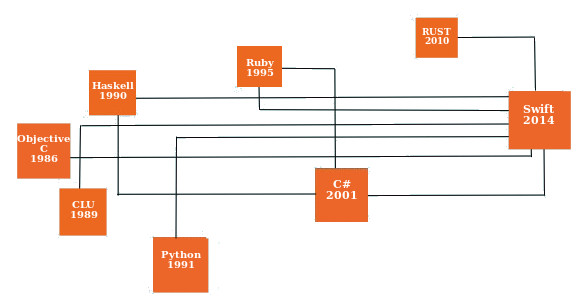
\includegraphics[scale=0.5]{razvojno_stablo.jpg}
\end{center}
\caption{Razvojno stablo}
\label{fig:razvojno_stablo}
\end{figure}

 Preuzeti su određeni delovi iz različitih programskih jezika i poboljšani. Pregled preuzetih koncepata se nalaze u tabeli \ref{tab:tabela2}.

\begin{table}[h!]
\begin{center}
\caption{Preuzeti koncepti iz drugih programskih jezika}
\begin{tabular}{|l|l|} \hline
\label{tab:tabela2}
Programski jezik & Šta je preuzeto \\ \hline
JavaScript & Struktura podataka - rečnik  \\ \hline
Scala i Opa & Zaključivanje tipova \\ \hline
Cold Fusion i JSP & Interpolacija Stringa \\ \hline
Python & Opciono naznačavanje kraja naredbe \\ \hline
Java i C\# & Protokoli (Interfejsi) \\ \hline
Lisp i Python & Tuples \\ \hline
Lisp i JavaScript &  Closure funkcije \\ \hline
C\# i Objective-C & Signed i unsigned int \\ \hline
\end{tabular}
\end{center}
\end{table}

\section{Osnovna namena, svrha i mogućnosti}	
\label{sec:drugiDeo}


Pomoću Swift programskog jezika moguće je razviti bilo koji tip iOS i macOS aplikacija. Cilj Swift projekta je da stvori najbolji raspoloživi jezik za upotrebu, od programiranja sistema, preko razvoja mobilnih i desktop aplikacija do cloud usluga. Takođe, ubrzan je proces razvoja proizvoda, poboljšane su performanse i povećana sigurnost aplikacija.

Jedna od glavnih namena Swift programskog jezika je kreiranje mobilnih aplikacija za iPhone i iPad uređaje. Swift je moguće izvršavati na Linux operativnom sistemu i Raspberry Pi. Članovi zajednice rade na stvaranju Swift aplikacija koje će se izvršavati i na Android platformama.

Osim što je Swift poznat po razvoju aplikacija za Apple platforme, koristi se i u modernim server aplikacijama. Swift je odličan izbor za server aplikacije koje zahtevaju visoke performanse kompajlera, nizak stepen korišćenja memorije i visok nivo bezbednosti.

Swift je sve popularniji programski jezik za razvoj IoT (eng.~{\em Internet of Things}) aplikacija. Kako bi kompanija Apple postala lider u primeni IoT aplikacija, razvijene su biblioteke i razvojni okviri koje rade najveći deo posla, dok se programeri mogu fokusirati na funcionalnosti IoT aplikacija.

Neka od mogućnosti koje pruža pomoću svojih funkcija \cite{mastering_swift3}
\begin{itemize}
\item Automatsko utvrđivanje tipova - Swift može automatski da utvrdi tip promenljive ili konstante na osnovu inicijalne
vrednosti. 
\item Generički tipovi - generički tipovi omogućavaju da se piše kod jednom za izvršenje identičnih
zadataka za različite tipove objekata dok se zadržava bezbednost tipa. 
\item Sintaksa zatvorenog izraza - zatvoreni izrazi su samostalni blokovi funkcionalnosti koji mogu da se proslede i upotrebe u kodu.
\item Pseudoklase - pseudoklasa definiše promenljivu koja možda nema vrednost.
\item Switch iskaz - Switch iskaz je drastično poboljšan funkcijama, kao što su poklapanje šablona i
zaštitni uslovi; zahvaljujući njima, izbegnute su automatske greške.
\item Višestruki povratni tipovi - funkcije mogu da imaju višestruke povratne tipove upotrebom torki. 
\item Preklapanje operatora - klase mogu da obezbede sopstvenu implementaciju postojećih operatora. 
\end{itemize}

Postoji još jedna funkcija, koja tehnički nije
funkcija Swifta, već Xcode-a i kompajlera. To je \textbf{Mix and match}. Ona omogućava kreiranje aplikacija koje sadrže Objective-C i Swift fajlove. To omogućava da se sistematski ažuriraju aktuelne Objective-C aplikacije pomoću Swift klasa i upotrebu Objective-C biblioteka/radnih okvira u Swift aplikacijama.

\section{Osnovne osobine programskog jezika}	
\label{sec:treciDeo}

Swift je objektno orijentisan programski jezik, koji je Apple razvio sa ciljem da 
se poboljšaju određeni delovi jezika Objective-C, ali da se i iskoriste njegove
dobre osobine. Najvažnije osobine programskog jezika Swift, koje ga čine izuzetnim za učenje iOS programiranja su \cite{swift_programming}:
\begin{itemize}
\item\textbf{Objektno orijentisan} - moderan objektno orijentisan jezik.
\item\textbf{Funkcionalan} - sadrži osobine zbog kojih je pogodan za pisanje funkcionalnih programa.
\item\textbf{Jasan} - lako se čita i lako piše, ima minimalne sintaksne ukrase i samo nekoliko skrivenih prečica. Njegova sintaksa je jasna, dosledna i očigledna.
\item\textbf{Bezbedan} - zahteva jake tipove kako bi obezbedio da u svakom trenutku i on i programer znaju na šta se sve tipovi objekata pozivaju.
\item\textbf{Ekonomičan} - mali jezik koji nudi samo neke osnovne tipove podataka i funkcionalnosti. Preostalo mora da bude dato kodom programera ili bibliotekama (razvojno okruženje Cocoa).
\item\textbf{Upravlja memorijom} - automatski upravlja memorijom, programer ne treba o tome da brine.
\item\textbf{Kompatibilnost sa razvojnim okruženjem Cocoa} -  Swift je napravljen tako da koristi većinu API interfejsa razvojnog okruženja Cocoa.
\end{itemize}

Zbog svih ovih osobina, 2016. godine, programski jezik Swift je bio najplaćeniji jezik u Americi. Na sledećem grafikonu (slika \ref{fig:grafikon}) prikazano je 10 najplaćenijih programskih jezika:

\begin{figure}[hbt!]

\begin{tikzpicture}
\pgfplotsset{width=10 cm, height = 5cm}
\begin{axis} [
symbolic x coords={Swift, Python, Ruby, C++, Java, JavaScript, C, SQL, PHP},
xtick={Swift, Python, Ruby, C++, Java, JavaScript, C, SQL, PHP},
x tick label style={rotate=45, anchor=east, align=center},
axis lines*=left,
ymajorgrids = true,
ylabel=Zarada u hiljadama,
legend style={at={(0.5,-0.10)},
    anchor=north,legend columns=1},
    ymin=80,
    ytick={80,90,...,120},
    ymax=120,
    bar width=5mm,
    ybar=-0.5cm, 
   enlarge x limits={abs=0.6cm},
    nodes near coords,        
    every node near coord/.append style={color=black},
]
\addplot [RYB3,fill=RYB3]
coordinates{ (Swift,115) } ;
\addplot [RYB2,fill=RYB2]
coordinates{ (Python,107) } ;
\addplot [RYB1,fill=RYB1]
coordinates{ (Ruby,107)  } ;
\addplot [RYB2,fill=RYB2]
coordinates{ (C++,104) } ;
\addplot [RYB2,fill=RYB2]
coordinates{ (Java,102) } ;
\addplot [RYB1,fill=RYB1]
coordinates{ (JavaScript,99) } ;
\addplot [RYB3,fill=RYB3]
coordinates{ (C,94)  } ;
\addplot [RYB1,fill=RYB1]
coordinates{ (SQL,92) } ;
\addplot [RYB3,fill=RYB3]
coordinates{ (PHP,89)  } ;

\end{axis}

\end{tikzpicture}
\caption{Najplaćeniji programski jezici u Americi 2016. godine}
\label{fig:grafikon}
\end{figure}

\subsection{Podržane paradigme}
\label{subsec:podnaslovParadigma}

Programski jezik Swift je objektno orijentisani jezik, ali podržava i funkcionalno i imperativno
programiranje. Sadrži sve osnovne koncepte objektno orijentisanog programiranja, i objektno orijentisana paradigma je najzastupljenija u ovom jeziku. Međutim, nekoliko osobina Swift jezika, kao što su funkcije prvog reda, sofisticirani sistem tipizacije, lambda izrazi, korišćenje Karijevih funkcija i parcijalna aplikacija, čine jezik posebno pogodnim za pisanje funkcionalnih programa\cite{rad}. Swift, kao funkcionalni jezik, može se u svakodnevnoj praksi koristiti za pisanje kraćih, elegantnijih i sigurnijih programa, koji su lakši za održavanje, nadogradnju i testiranje.

\section{Okruženja i njihove karakteristike}	
\label{sec:cetvrtiDeo}
Programski jezik Swift se može pisati u različitim okruženjima. Najpoznatije okruženje je \textbf{Xcode}, a pored njega, koriste se i AppCode, Atom, CLion, SublimeText.

\subsection{Xcode}
\label{subsec:podnaslovXcode}
Xcode  je integrisano razvojno okruženje koje je napravila kompanija Apple. Koristi se za razvoj iOS i macOS aplikacija. U ovom okruženju mogu se pisati kodovi u mnogim programskim jezicima, kao što su C, C++, Objective-C, Java, AppleScript, Python, Ruby i Swift. Xcode sadrži i okvire, za programski jezik Swift su najvažniji \textbf{Playground} i \textbf{Cocoa Touch}. 
Postoji 9 verzija ovog okruženja, a od verzije 6, obuhvata i programski jezik Swift.


\subsection{Playground}
\label{subsec:podnaslovPlayground}
Playground  je interaktivno radno okruženje koje omogućava da pišemo kod i odmah vidimo rezultate čim su promene izvršene u kodu. Kako bismo mogli da koristimo ovaj okvir potrebno je prvo da pokrenemo Xcode i zatim izaberemo opciju Get started with a playground.
Sastoji se od nekoliko delova, među kojima su najvažniji: 
\begin{itemize}
\item Prostor za kodiranje.
\item Bočna traka za rezultate.
\item Prostor za ispravljanje grešaka.
\end{itemize}


\subsection{SublimeText}
\label{subsec:podnaslovSublimeText}

Sublime Text  je verovatno jedan od najrasprostranjenijih okruženja. Poseduje dobar korisnički interfejs i sjajne performanse. On u osnovni podržava mnoge programske jezike a nove funkcionalnosti mogu biti dodate korišćenjem dodataka (plugina), koji je zajednica razvijala pod licencom slobodnog softvera. Vrlo lako ga možemo prilagoditi za razvoj Swift aplikacija dodatkom podrške za Swift pakete.


\subsection{Atom}
\label{subsec:podnaslovAtom}
Atom je razvijen od strane GitHub-a, visoko modularno okruženje koje omogućava laku instalaciju novih paketa što ga je svrstalo među najpoželjnija okruženja. Dodavanje podrške za Swift programiranje je jednostavno instaliranjem language-swift paketa.



\section{Instalacija i uputstvo za pokretanje}	
\label{sec:petiDeo}

Programski jezik Swift se može koristiti na različitim operativnim sistemima. Ukoliko koristimo MAC operativni sistem, dovoljno je da se preuzme i instalira Xcode razvojno okruženje, jer Xcode uključuje izdanje Swift-a koje podržava Apple. Za Linux i Windows instalacija i pokretanje su složeniji, i biće prikazano u ovom poglavlju.

\subsection{Swift na Windows-u}
\label{subsec:podnaslovWindows}

Za instalaciju jezika Swift na Windows-u potrebno je prvo da ga preuzmemo sa ovog \href{https://swiftforwindows.github.io}{linka}. Nakon toga nam se pojavljuje prozor za instalaciju, gde pratimo dalja uputstva i tako instaliramo Swift i kompajler za ovaj jezik. Nakon završetka instalacije, potreban nam je editor teksta u kojem želimo da kodiramo. Možemo koristiti bilo koje od gore navedenih razvojnih okruženja u kojem nam je udobno da radimo. U ovom primeru koristićemo \href{https://notepad-plus-plus.org/download/v7.6.4.html}{Notepad++}, koji je jednostavan, besplatan i lak za instalaciju.


Nakon instalacije okruženja, napisaćemo jednostavan program koji ćemo kasnije pokrenuti pomoću Windows komandne linije. Prvo je potrebno da otvorimo novi Notepad++ fajl, i u njega unosimo komandu za ispis.



\begin{lstlisting}[language=bash, caption={Primer komande}]
print("Hello world!")
\end{lstlisting}

Da bi sačuvali ovaj kod, koristićemo File > Save As i izabrati Swift file iz Save As Type menija. Ako u meniju nedostaje tip ovog fajla izabraćemo all files, i dodati .swift fajl ekstenziju nakon što smo dali odgovarajuće ime fajlu.

Sada kada imamo program, želimo da ga kompajliramo i pokrenemo. Za kompajliranje i pokretanje koristimo korisnički interfejs Swift-a koji je prikazan na slici \ref{fig:windows}.

\begin{figure}[h!]
\begin{center}
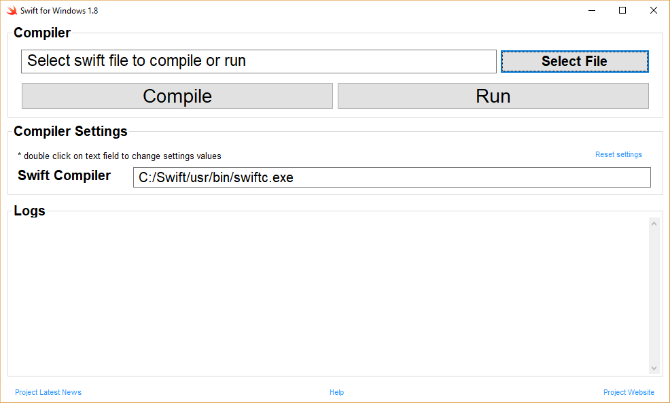
\includegraphics[scale=0.35]{swift-win.png}
\end{center}
\caption{Korisničko okruženje za Windows}
\label{fig:windows}
\end{figure}


Nakon pritiska na Select File izabraćemo naš program koji smo prethodno napisali i pritisnuti Compile. Nakon što sačekamo da se kompilacija završi dobićemo poruku “Successfully compiled”.
Jednom kompajliran program možemo pokrenuti neograničen broj puta.

\subsection{Swift na Linux-u}
\label{subsec:podnaslovLinux}

Kao i u prethodnom primeru biće nam potreban tekst editor gde ćemo napisati jednostavan kod.
Možemo koristiti bilo koji integrisani editor koji Linux poseduje. Na isti način ćemo iskodirati poruku za ispis "Hello World", kao u prethodnom primeru, i taj fajl ćemo sačuvati sa ekstenzijom .swift.

Da bismo koristili Swift na Linux-u moramo ga prvo instalirati. U terminalu kucamo sledeće komande:

\begin{lstlisting}[language=bash, caption={Instaliranje Swift-a}]
	wget https://swift.org/builds/ubuntu1510/swift-2.2-SNAPSHOT-2015-12-10-a/swift-2.2-SNAPSHOT-2015-12-10-a-ubuntu15.10.tar.gz

\end{lstlisting}
Nakon preuzimanja, pozicioniraćemo se u folder Downloads i tamo raspakovati arhivu u kojoj se nalazi Swift instalacija.

\begin{lstlisting}[language=bash, caption={Raspakovanje Swift instalacije}]
  cd ~/Downloads
  tar -xvzf swift-2.2-SNAPSHOT*
\end{lstlisting}

Kada raspakujemo fajl potrebno je podesiti putanju do BIN-a kako bismo mogli da izvršavamo programe.

\begin{lstlisting}[language=bash, caption={Podešavanje putanje do BIN-a}]
  cd ~/Downloads/swift-2.2-SNAPSHOT*
  cd usr/bin
  pwd
\end{lstlisting}

Kao rezultat komande pwd dobićemo tačnu lokaciju koju ćemo koristiti. Kopiramo i zamenimo je na sledeći način.
\begin{lstlisting}[language=bash, caption={Kopiranje putanje}]
  export PATH=path_to_swift_usr_bin:$PATH

\end{lstlisting}

Zatim moramo instalirati jos par biblioteka kako bi omogućili da Swift nesmetano funkcioniše na Linux-u.

\begin{lstlisting}[language=bash, caption={Instalacija biblioteka}]
  sudo apt-get install clang libicu-dev
  swift -version
\end{lstlisting}

Na kraju, da bismo kompajlirali i pokrenuli prethodno napisan program potrebno je da ukucamo sledeće komande:

\begin{lstlisting}[language=bash, caption={Komanda za kompajliranje}]
  swift imeprograma.swift
  ./imeprograma
\end{lstlisting}


\section{Primer jednostavnog koda i njegovo objašnjene}	
\label{sec:sestiDeo}

U narednim primerima biće prikazane i objašnjene osnovne funkcionalnosti jezika Swift.
\begin{primer}

Ispis teksta se vrši pomoću funkcije print(). Tačka-zarez su opcioni na kraju svakog reda.
\end{primer}

\begin{lstlisting}[language=Swift, caption={Ispis teksta},frame=single, label=simple]
print("Hello world!")
print("Hello world!");

\end{lstlisting}

\begin{primer}
Stringovi se takodje dodeljuju pomoću operatora dodele. Konkatenacija stringova se vrši pomoću specijalnih karaktera '$\backslash$ (string)' ili jednostavnim navodjenjem u naredbi 'print', gde se stringovi razdvajaju zarezima.
\end{primer}

\begin{lstlisting}[language=Swift, caption={Stringovi i konkatenacija stringova},frame=single, label=simple]
var ime = "Swift"
var jezik = "programski jezik"

var poruka = " je najbolji "
var poruka1 = "\ (ime) je najbolji \ (jezik) !" 

print(ime,poruka,jezik,"!")
print(poruka1)

\end{lstlisting}

\begin{primer}
Listu stringova koji su razdvojeni određenim separatorom, pravimo pomoću naredbe print, gde se prvo navode stringovi koji čine tu listu, a nakon toga separator i terminator. Možemo koristiti jos jedan parametar u funkciji print(), pod nazivom toStream. Pomoću njega preusmeravamo ispis funkcije print(). Konkretno u ovom primeru preusmeravamo ispis u promenljivu ime4.
\end{primer}
\begin{lstlisting}[language=Swift, caption={Lista stringova},frame=single, label=simple]
var ime1 = "Swift"
var ime2 = "Java"
var ime3 = "Python"
var ime4 = ""

print(ime1,ime2,ime3,separator:", ", terminator:"")
print(ime1,ime2,ime3,separator:", ", terminator:"", to:&ime4)

\end{lstlisting}

\begin{primer}
U ovom primeru je pokazana funkcionalnost for i while petlje. Takođe jos jednom i mogućnost konkatenacije pomoću operatora +. Nakon for petlje u konzoli će biti ispisani brojevi od 0 do 10. U while petlji će se svakog puta dodavati po jedno slovo a, i tako 5 puta.
\end{primer}

\begin{lstlisting}[language=Swift, caption={Petlje},frame=single, label=simple]
var x:Int = 0
for x in 0...10 {
	print(x)
}

var y:String = ""
while y != "aaaaa" {
	print(y)
	y = y + "a"
}

\end{lstlisting}

\begin{primer}
Pozivanje funkcije sa parametrima koja nema povratnu vrednost. Sintaksa za deklaraciju funkcija se sastoji iz ključne reči func, naziva i liste parametara. Parametri su oblika naziv ':' tip promenljive.
\end{primer}

\begin{lstlisting}[language=Swift, caption={Funkcije bez povratne vrednosti},frame=single, label=simple]
var skor:Int = 0
var trenutno_stanje:Float = 0

func dodaj_poene_i_novac(poeni:Int, novac:Float){
	skor = skor + poeni
	trenutno_stanje = trenutno_stanje + novac
}

dodaj_poene_i_novac(poeni: 30, novac: 1.45)
dodaj_poene_i_novac(poeni: 60, novac: 2.86)

print(skor)
print(trenutno_stanje)

\end{lstlisting}

\begin{primer}
Funkcije u programskom jeziku Swift dozvoljavaju da vraćamo jednu ili više vrednosti istovremeno. Sintaksa za povratnu vrednost je 'return(niz vrednosti koje želimo da vratimo)'.
\end{primer}

\begin{lstlisting}[language=Swift, caption={Funkcije koje imaju povratnu vrednost},frame=single, label=simple]
func izracunajMinMaxSuma(a: Int, b: Int) -> (min: Int, max: Int, suma: Int) {
    
    if a > b {
        return (b, a, a + b)
    } else {
        return (a, b, a + b)
    }
}
let statistika = izracunajMinMaxSuma(5, b: 19)
let (min2, max2, suma2) = izracunajMinMaxSuma(5, b: 19)
print(suma2)            
print(statistika.sum)   
print(statistika.2)     

\end{lstlisting}


\section{Specifičnosti}	
\label{sec:sedmiDeo}

Swift je veoma pristupačan novim programerima, to je industrijski kvalitetan programski jezik koji je veoma detaljan i pogodan kao skriptni jezik. Swift se dobro štiti od najzastupljenih programskih grešaka usvajanjem modernih paterna programiranja:
\begin{itemize}
\item Promenjive su uvek inicijalizovane pre upotrebe.
\item Obrađena je greška za pristupanje nepostojećem elementu niza (eng.~{\em out of bounds}).
\item Integer-i su provereni za prekoračenje memorije (eng.~{\em overflow}).
\item Opcione promenjive zahtevaju eksplicitno rukovanje.
\item Memorijom se upravlja automatski.
\item Rukovanje greškama omogućava kontrolisani oporavak od neočekivanih prekida (crash).
\end{itemize}

Swift kod je kompajliran i optimizovan da izvuče najviše iz modernog hardvera. Sintaksa i standardna biblioteka su bazirane na konceptu da je očigledan način za pisanje koda takav da se on izvršava najbolje. Ova kombinacija sigurnosti i brzine čini Swift odličnim izborom za sve, od komande "Hello world!", do celog operativnog sistema.

\section{Zaključak}
\label{sec:zakljucak}
Swift je mlad jezik, koji iz godine u godinu napreduje i postaje popularniji u iOS programiranju. Očekuje se njegova ekspanzija u narednom periodu, pre svega zbog sve većeg korišćenja iOS aplikacija. Godinama se radilo na Swift-u i on nastavlja da evoluira sa novim funkcionalnostima, a cilj koji ima je veoma ambiciozan. Ovaj seminarski rad ima za cilj da uvede čitaoca u ovaj jezik, a takodje, i da ga motiviše da nastavi sa učenjem i usavršavanjem ovog jezika. 

\addcontentsline{toc}{section}{Literatura}
\appendix
\bibliography{seminarski} 
\bibliographystyle{plain}

\appendix

\end{document}